\documentclass[a4paper]{article}

%use the english line for english reports
%usepackage[english]{babel}
\usepackage[portuguese]{babel}
\usepackage[utf8]{inputenc}
\usepackage{indentfirst}
\usepackage{graphicx}
\usepackage{verbatim}
\usepackage{url}


\begin{document}

\setlength{\textwidth}{16cm}
\setlength{\textheight}{22cm}

\title{\Huge\textbf{Aplicação em Prolog para um Jogo de Tabuleiro}\linebreak\textbf{Cequis - Sumo}\linebreak\linebreak
\Large\textbf{Relatório Intercalar}\linebreak\linebreak

\includegraphics[height=6cm, width=7cm]{feup.pdf}\linebreak \linebreak
\Large{Mestrado Integrado em Engenharia Informática e Computação} \linebreak \linebreak
\Large{Programação em Lógica}\linebreak
}

\author{\textbf{Grupo 45:}\\ Duarte Duarte - ei11101 \\ Hugo Freixo - ei11086 \\\linebreak\linebreak \\
 \\ Faculdade de Engenharia da Universidade do Porto \\ Rua Roberto Frias, s\/n, 4200-465 Porto, Portugal \linebreak\linebreak\linebreak
\linebreak\linebreak\vspace{1cm}}
%\date{Junho de 2007}
\maketitle
\thispagestyle{empty}

\newpage

\section*{Resumo}
Neste trabalho pretende-se implementar o jogo de tabuleiro Cequis - Sumo, na linguagem de programação Prolog. A aplicação permitirá 2 jogadores defrontarem-se em 3 modo distintos: humano/humano, humano/computador e computador/computador. A aplicação terá também um visualizador gráfico 3D implementado em C++ (no âmbito da cadeira de LAIG).

\section{}
\tableofcontents

\newpage

\section{Introdução}
Este trabalho tem como objetivo o aprofundamento dos conhecimentos em programação em lógica, para isso iremos criar o jogo Cequis - Sumo utilizando a linguagem programação lógica Prolog.

O grupo escolheu este tema pois simular o jogo Cequis - Sumo em programação lógica mostrou ser bastante desafiador, além disso as jogadas possíveis de efetuar são imensas, tornando o jogo uma verdadeira batalha mental para os jogadores.
Há que notar várias caraterísticas que tornam este jogo diferente de muitos outros jogos de tabuleiro:

\begin{itemize}
\item O tabuleiro não é regular, em vez de ser constituído por quadrados é constitiuído por hexagonos.
\item Existe um pedra neutra que ambos os jogadores podem movimentar utilizando as próprias pedras para o efeito.
\item É possível movimentar as pedras do adversário através das próprias pedras.
\end{itemize}

\section{O Jogo Cequis - Sumo}

Cequis - Sumo é um jogo de tabuleiro disputado entre dois adversários, que possuem três pedras cada.
O seu objetivo é retirar a pedra objetivo (ou branca) da mesa, empurrando-a para fora do tabuleiro, antes que o jogador adversério o faça.
O tabuleiro consiste num conjunto de hexágonos ligados entre si desta forma: 

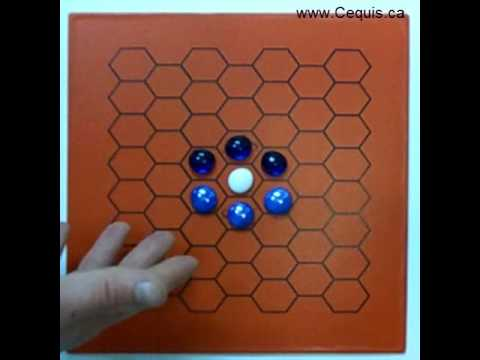
\includegraphics[height=4cm, width=5cm]{sumo.jpg}

Os jogadores podem andar para cima, baixo, cima-direita, cima-esquerda, baixo-direita e baixo-esquerda e só podem efectuar um movimento por jogada.

O jogador pode mover uma peça ou um conjunto de peças. Um conjunto de peças são peças da mesma cor que estão em espaços adjacentes.

É possivel empurrar pedras adversárias, sem as retirar do tabuleiro, mas para isso é necessário um número maior ou superior de pedras que o número de pedras que vamos empurrar. Podemos empurrar a pedra objectivo juntamente com pedras adversárias, neste caso a pedra objectivo não tem "peso", ou seja não é necessário uma pedra extra para a empurrar, apenas precisamos de cobrir o número de pedras do nosso adversário que queremos empurrar.

\section{Representação do Estado do Jogo}
O estado do tabuleiro será representado em Prolog recorrendo a uma lista de listas de peças válidas com a adição de uma peça fictícia para assinalar um espaço no tabuleiro sem peças.

\begin{itemize}
\item b - black - peça do jogador 1
\item w - white - peça do jogador 2
\item o - objective - peça objetivo
\item e - empty - posição sem peça
\end{itemize}

Estado inicial (tabuleiro de tamanho 8):
\begin{verbatim}
[[e,    e,    e,    e],
 [e, e, e, e, e, e, e],
 [e, e, e, e, e, e, e],
 [e, e, w, w, w, e, e],
 [e, e, b, o, b, e, e],
 [e, e, e, b, e, e, e],
 [e, e, e, e, e, e, e],
 [e, e, e, e, e, e, e]]
\end{verbatim}

Possível estado intermédio (tabuleiro de tamanho 8):
\begin{verbatim}
[[e,    e,    e,    e],
 [e, e, e, e, e, e, e],
 [e, e, e, e, e, e, o],
 [e, e, w, w, b, w, e],
 [e, e, b, e, b, b, e],
 [e, e, e, e, e, e, e],
 [e, e, e, e, e, e, e],
 [e, e, e, e, e, e, e]]
\end{verbatim}

Possível estado final (tabuleiro de tamanho 8):
\begin{verbatim}
[[e,    e,    e,    e],
 [e, e, e, e, e, e, e],
 [e, e, e, e, e, e, w],
 [e, e, e, w, b, w, e],
 [e, e, b, e, b, e, e],
 [e, e, e, e, e, e, e],
 [e, e, e, e, e, e, e],
 [e, e, e, e, e, e, e]]
\end{verbatim}


\section{Visualização do Tabuleiro}
A visualização do tabuleiro em modo de texto é feita através da composição de caracteres ASCII. Para tal foi desenvolvido um conjunto de predicados, sendo show\_board/1 (que aceita uma lista de listas de peças por argumento) o predicado principal. Os predicados auxiliares são: draw\_piece/1, draw\_letters/1, draw\_letters\_aux/1, draw\_line\_numbers/1, draw\_slashes/1, draw\_lower\_cell/1, show\_line/2 e show\_piece/2.

A função show\_board/1 é génerica, ou seja, funciona com qualquer tamanho de tabuleiro (desde que a lista de listas de peças fornecidas seja válida).

O código destes predicados encontra-se em anexo.

Imagem do output produzido por show\_board/1:

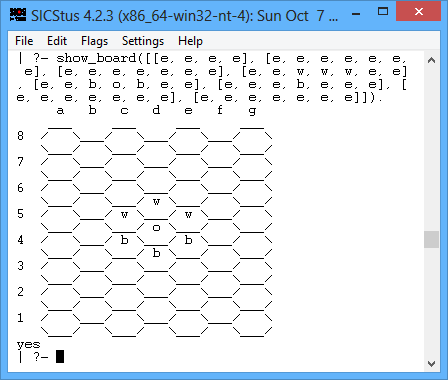
\includegraphics[height=6cm, width=7cm]{screenshot.png}

\section{Movimentos}
Sendo o nosso tabuleiro um tabuleiro especial e devido ao facto de utilizarmos uma lista de listas para guardar o estado do jogo, o movimento das pedras precisará de alguns predicados auxiliares.
Utilizaremos um predicado para verificar se a casa para a qual queremos mudar é adjacente à casa inicial:

\begin{itemize}
\item adjacent (Line, Column, LineTo, ColumnTo).
\end{itemize}

Também usaremos um predicado para verificar se naquela posição da lista existe uma pedra e caso exista, que tipo de pedra é (b, w, o, e):
\begin{itemize}
\item object(Line, Column, X).
\end{itemize}
%------------
O nosso predicado de movimentar pedras será:

\begin{itemize}
\item valid\_move(Line, Column, LineTo, ColumnTo).
\end{itemize}

Esta função deve mover a pedra que esta em Line Column para LineTo ColumnTo e caso já exista uma pedra em LineTo ColumnTo verificar se é possível empurrar essa pedra, caso seja o movimento é efectuado, caso contraria a função devolve \textit{no}.


\section{Conclusões e Perspectivas de Desenvolvimento}
Em suma, o trabalho em desenvolvimento antingirá os objetivos pretendidos de forma satisfatória.
Vendo as impressões do tabuleiro já obtidas, podemos já visualizar a estrutura que terá o jogo futuramente.

Ainda não é possível a realização de um jogo de qualquer forma, mas o grupo prevê que isso se tornará possível num período próximo.

Feito um balanço da situação atual do trabalho o grupo estima que o trabalho esteja 15\% concluído.

\clearpage
\addcontentsline{toc}{section}{Bibliografia}
\renewcommand\refname{Bibliografia}

\begin{thebibliography}{9}

\bibitem{cequis}
  cequis.ca,
  \url{http://www.cequis.ca/variations/Sumo.php/},
  13 10 2013.

\end{thebibliography}

\newpage
\appendix
\section{Código Prolog}
\begin{verbatim}
%%  Prolog implementation of Cequis - Sumo   %%
%%        FEUP - MIEIC - 2013/2014           %%
%%                                           %%
%% Authors:                                  %%
%% + Duarte Duarte - ei11101@fe.up.pt        %%
%% + Hugo Freixo   - ei11086@fe.up.pt        %%
%%                                           %%
%%      a   b   c   d   e   f   g            %%
%%     ___     ___     ___     ___           %%
%% 8  /   \___/   \___/   \___/   \          %%
%%    \___/   \___/   \___/   \___/          %%
%% 7  /   \___/   \___/   \___/   \          %%
%%    \___/   \___/   \___/   \___/          %%
%% 6  /   \___/   \___/   \___/   \          %%
%%    \___/   \___/ w \___/   \___/          %%
%% 5  /   \___/ w \___/ w \___/   \          %%
%%    \___/   \___/ o \___/   \___/          %%
%% 4  /   \___/ b \___/ b \___/   \          %%
%%    \___/   \___/ b \___/   \___/          %%
%% 3  /   \___/   \___/   \___/   \          %%
%%    \___/   \___/   \___/   \___/          %%
%% 2  /   \___/   \___/   \___/   \          %%
%%    \___/   \___/   \___/   \___/          %%
%% 1  /   \___/   \___/   \___/   \          %%
%%    \___/   \___/   \___/   \___/          %%
%%                                           %%
%% [[e,    e,    e,    e],                   %%
%%  [e, e, e, e, e, e, e],                   %%
%%  [e, e, e, e, e, e, e],                   %%
%%  [e, e, w, w, w, e, e],                   %%
%%  [e, e, b, o, b, e, e],                   %%
%%  [e, e, e, b, e, e, e],                   %%
%%  [e, e, e, e, e, e, e],                   %%
%%  [e, e, e, e, e, e, e]]                   %%
%%                                           %%
%%  b - black (P1 pieces)                    %%
%%  w - white (P2 pieces)                    %%
%%  e - empty (nothing)                      %%
%%  o - objective (objective piece)          %%
%%                                           %%
%% http://www.cequis.ca/variations/Sumo.php  %%
%%                                           %%

library(lists).
% use_module(library(lists)).

%% board representation - main method is show_board(B) %%

show_board(B) :-
    length(B, N),
    Nm1 is N - 1,
    No2 is N // 2,
    write('    '), draw_letters(Nm1), nl,
    write('  '), draw_slashes(No2), nl,
    show_line(B, 0),
    write('  '), draw_lower_cell(No2), nl.

draw_piece(b) :- write(' b ').
draw_piece(w) :- write(' w ').
draw_piece(o) :- write(' o ').
draw_piece(e) :- write('   ').
draw_piece(N) :- write(' '), write(N), write(' ').

letters([a, b, c, d, e, f, g, h, i, j, k, l, m, n, o, p, q, r, s, t, u, v, w, x, y, z]).

draw_letters(N) :-
    letters(L),
    sublist(L, SL, 0, N, _),
    draw_letters_aux(SL).

draw_letters_aux([]).
draw_letters_aux([H|T]) :-
    write(' '), write(H), write('  '),
    draw_letters_aux(T).

draw_line_number(N) :-
    N >= 0,
    N < 10,
    write(N), write('  ').
draw_line_number(N) :-
    N >= 10,
    N < 100,
    write(N), write(' ').
draw_line_number(N) :-
    N >= 100,
    N < 1000,
    write(N).

draw_slashes(0).
draw_slashes(N) :-
    write('  ___   '),
    N1 is N - 1,
    draw_slashes(N1).

draw_lower_cell(0).
draw_lower_cell(N) :-
    write(' \\___/  '),
    N1 is N - 1,
    draw_lower_cell(N1).

show_line([], _).
show_line([BH|BT], LINEN) :-
    even(LINEN),
    LINEN1 is LINEN + 1,
    length([BH|BT], X),
    draw_line_number(X),
    show_piece(BH, LINEN, 0), nl,
    show_line(BT, LINEN1).
show_line([BH|BT], LINEN) :-
    odd(LINEN),
    LINEN1 is LINEN + 1,
    write('   '),
    show_piece(BH, LINEN, 0), nl,
    show_line([BH|BT], LINEN1).

show_piece([], _, _).
show_piece(L, 0, PIECEN) :-
    odd(PIECEN),
    write('___'),
    PIECEN1 is PIECEN + 1,
    show_piece(L, 0, PIECEN1).
show_piece([LH|LT], LINEN, PIECEN) :-
    even(LINEN),
    even(PIECEN),
    write('/'), draw_piece(LH), write('\\'),
    PIECEN1 is PIECEN + 1,
    show_piece(LT, LINEN, PIECEN1).
show_piece([_|LT], LINEN, PIECEN) :-
    even(LINEN),
    odd(PIECEN),
    write('___'),
    PIECEN1 is PIECEN + 1,
    show_piece(LT, LINEN, PIECEN1).
show_piece([_|LT], LINEN, PIECEN) :-
    odd(LINEN),
    even(PIECEN),
    write('\\___/'),
    PIECEN1 is PIECEN + 1,
    show_piece(LT, LINEN, PIECEN1).
show_piece([LH|LT], LINEN, PIECEN) :-
    odd(LINEN),
    odd(PIECEN),
    draw_piece(LH),
    PIECEN1 is PIECEN + 1,
    show_piece(LT, LINEN, PIECEN1).

%% helpers %%

even(N) :- N mod 2 =:= 0.
odd(N) :- \+ even(N).

%% show_board([[e, e, e, e], [e, e, e, e, e, e, e], [e, e, e, e, e, e, e], [e, e, w, w, w, e, e], [e, e, b, o, b, e, e], [e, e, e, b, e, e, e], [e, e, e, e, e, e, e], [e, e, e, e, e, e, e]]).

\end{verbatim}

\end{document}
